% !TEX root = ../../report.tex

\section{State Of The Art}

The following section will present the state of the art recommender systems...

\subsection{System Cold-start Handling}

In the literature, the term cold is used about an object in a system, or a
whole system, which is new. Cold-start scenarios in recommender systems are
situations in which little/no prior events, like ratings or clicks, are known
for certain users or items. The cold-start problem can therefore be divided into three sub problems:

\begin{itemize}
  \item \emph{Cold-start system}: A situation where we only have new users and
  little or no ratings for the items.

  \item \emph{Cold-start item}: The problem of recommending items that are new
  to the system, which have not received any ratings. 

  \item \emph{Cold-start user}: The problem of giving accurate recommendations
  who is new to a recommender system.
\end{itemize}

For example in a scenario where the average item in an item collection have 5 000 ratings, a new item with only 5 ratings would be considered an "cold-item". Likewise, in a recommender system where the average user have rated 25 items, a user which only have rated 2 items, would be considered a "cold-user".

The cold-start system problem is mainly a collaborative filtering problem, and
can be seen as a combination of the cold-start user and cold-start item problem
where the majority of the users are new to the system and have expressed few
preferences, resulting in a very sparse user-item matrix, rendering
recommendation systems using traditional collaborative-filtering methods
futile.

In content-based systems, new items can easily be
recommended using the content information of the item, making it a popular
solution to the cold-start new item problem. This problem is more
severe in collaborative-filtering systems where items are only recommendable if
they have been rated by substantial amount of users. New items will therefore not be
recommendable before multiple users somehow stumble upon the new item while
e.g. browsing the item collection, unless additional measures are taken to
solve this problem. To solve the new-item problem, there are two commonly used (simple) solutions
that often are used in E-commerce websites:

\begin{itemize}
\item Advertising at the homepage/front-page of the website, putting the new
items in an eye catching position. This solution, however, may this result in
that some users, which don't like these new items, might leave the website.
\item Requesting the user to choose one or more of his/hers categories while
registering for the site, and recommend items from the selected categories.
This approach however, requires active user involvement and complicates the
sign up process. Many users might chose not to give up any
personal interest information, thus the user group covered by this solution could end up not being large enough.
\end{itemize}

Another crucial problem of recommender system is how to best learn from new users.
Collaborative Filtering (CF), is the best known technology for recommender
systems and is based on the idea that like-minded users have similar tastes and
preferences. A new user therefore poses a challenge to CF recommender, since
the system has no knowledge about the preferences of the new user, and can
therefore not provide any personalized recommendations, this is known as the
cold start problem for new users. The system must therefore acquire some
information about the new user in order to make personalized recommendations.

The cold-start user problem is present both in content-based and
collaborative-filtering systems. In content-based systems, the lack of ratings
given by the target user, means that the target user will have a limited
content-profile, since the users content profile is constructed using
content-information from his/hers rated items. Similarly, the cold-start user
problem also affects user-based collaborative filtering, since user
similarities are calculated based on items that a user shares with other users
of the system. In a typical domain, for example in the domain of books, the number of items is very large (in the order of tens of thousands) while the number of items rated by every single user is in general small (in the order of dozens or less). This means that it is very unlikely two random users have rated any items in common and hence they are not comparable. The system will therefore most likely struggle to find users
with tastes that are \emph{truly} similar to the target user. In both cases, recommendation quality is most likely bound to suffer.
		
In this section we will present a few different solutions to the cold-start problem, focusing mainly on \emph{complete} solutions to the cold-start problem and all the sub problems. Most traditional algorithms only work effectively in environments where
the datasets has high information density. In fact, in extreme cases, when data
is very scarce, simple non-personalized recommendations based on global
averages can outperform collaborative-filtering and content-based algorithms.
Pure collaborative filtering cannot help in a cold-start setting, since no user
preference information is available to form any basis for recommendations

%Can the different approaches be classified? E.g. 3 main categories of approaches
	%Initial categorization
		%Interview process
 		%Hybrid approaches
 		%Key figures / Seed users
 		%Filterbots
 		%Trust-aware / Trust propagation


\subsubsection{Trust Aware Recommender Systems}

Due to the popularity of social networks such as Facebook, more and more
researchers turn to incorporate the social relationships (e.g. trust) of users
to help complement users’ preference in addition to item ratings, in order to overcome the limitations of existing recommender systems. For example, when looking for movie recommendations we often turn to our friends which we share a similar taste in movies with. Trust can be defined as: "believe in the reliability, truth, or ability of", and in the context of recommender systems a trusted user would be a user you trust to provide you good recommendations. Trust relationships of users are often employed in order to correlate more potential raters for the active users who require recommendations. Massa et. al. \citep{Massa2004} show that some of the weaknesses of RS such as data sparseness and their susceptibility to shilling attacks could be alleviated by incorporating trust.

% Web of Trust - Figure explanation
Using explicit trust statements, it is possible to predict trust in unknown
users by propagating trust. Consider the example shown in Figure
\ref{figure:weboftrust}. User A has issued a trust statement in B and C; hence
B and C are in the web of trust of A. Using these explicit trust statements, it
is possible to predict trust in unknown users by propagating trust, making it
possible to infer something about how much user A could trust D.

\begin{figure}[H]
    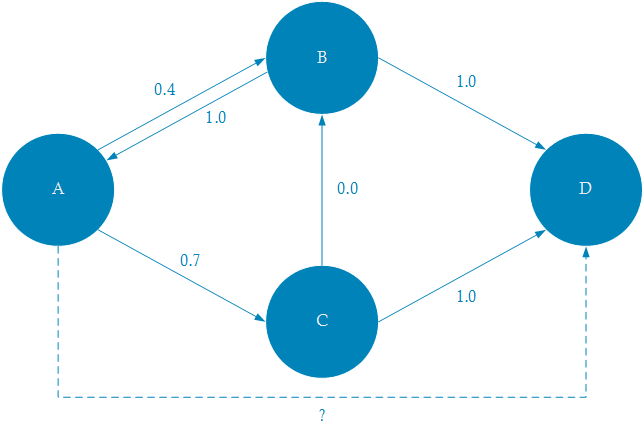
\includegraphics[width=5in]{image/webofTrust.png}
    \centering
    \caption[Trust Network]{Trust Network. Nodes are users and solid edges are trust statements. The dotted edge is one of the undefined and predictable trust statements (Adopted from \cite{Massa2004}}
    \label{figure:weboftrust}
\end{figure}

% The formals
To capture all the trust statements we need a $NxN$ matrix, where $N$ is the
number of users, since each user is allowed to express a trust value in every
other user. This matrix will make up our trust network among the users. If $u$
trusts $v$, then there is a value $t_{u,v}$ for this trust which is a real
number in $[0,1]$. Zero means no trust and one means full trust. In addition to
the trust network we will also have a Rating matrix of size $NxM$, where $M$ is
the number of items. This rating will not differ from a standard rating matrix,
which are used in traditional collaborative filtering systems. The value $r_{u,
i}$, is the rating user $u$ have given to item $i$, the rating scale may differ
from system to system.

% Architecture
The systems takes as input the trust network (representing the trust
statements) and the ratings matrix (ratings given by users to items) and
produces, as output, a matrix of predicted ratings that the users would assign
to the items. Figure \ref{figure:trustarThe cold-start system problem is mainly a collaborative filtering problem, and
can be seen as a combination of the cold-start user and cold-start item problem
where the majority of the users are new to the system and have expressed few
preferences, resulting in a very sparse user-item matrix, rendering
recommendation systems using traditional collaborative-filtering methods
futile.chictecture} shown a conceptual
overview of the trust-aware recommender system architecture.

\begin{figure}[H]
    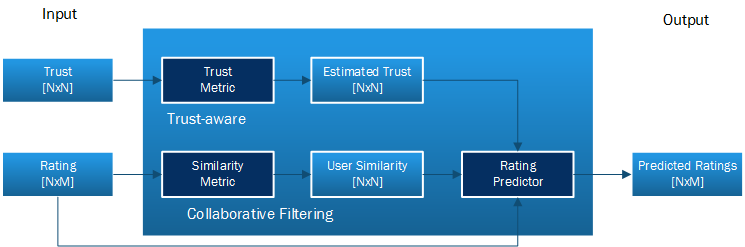
\includegraphics[width=5in]{image/trustawarearchitecture.png}
    \centering
    \caption[Trust-Aware Recommender System Architecture]{Trust-Aware
    Recommender System Architecture. Adopted from \cite{Massa2004}}
    \label{figure:trustarchictecture}
\end{figure}

The \emph{Trust Metric} module takes the trust network as input, and exploits
trust propagation in order to predict, for every user, how much she could trust
other users. Trust metrics can either be local and global. Global trust metrics
produces an estimated trust matrix with all the rows equal, meaning that the
estimated trust in a certain user (column) is the same for every user (row). A
simple local trust metric could e.g. for each user assign to every other user a
predicted trust based on her minimum distance from the source user. More
sophisticated ones could also be employed. If we again consider Figure
\ref{figure:weboftrust}, we could employ a local trust metric where the
predicted trust is based on the minimum distance from the source user. If we
set the maximum propagation distance $d$, a user at distance $n$ from the
source user will have a predicted trust value of:

\begin{equation}
t_{u,v} = (d-n+1)/d
\end{equation}

Giving users not reachable within the maximum propagation distance a trust of
$0$. Using user $A$ as the source user, the users at distance $1$ ($B$ and $C$)
would get a trust value of $(4-1+1)/4 = 1$, while the user at distance 2 (D)
would get a predicted trust value of $(4-2+1)/4 = 0.75$. Meaning that we will
have a linear decay in trust based on the distance from the source user.

The \emph{Similarity Metric} module computes the user similarities, this is one
of the standard steps of any traditional collaborative filtering technique,
user similarities can be found e.g. by using the Pearson Correlation
Coefficient. The intuition is that, if a user rates in a similar way to another
user, then her ratings are using for predicting the ratings for that users.

The \emph{Rating Predictor} can use the neighbors from the user similarity
matrix, the estimated trust matrix or a combination of both in order to
calculate the predicted ratings.

The main advantage is not improved accuracy, but improved coverage. As
exemplified by Massa et. al. \cite{Massa2007}. The authors experimented with
propagating the trust up to a distance of 4. By using the Pearson Correlation
coefficient they found on average 160.73 neighbors. However just propagating a
few steps help to increase significantly the number of neighbors that can be
considered for rating predictions. Propagating at distance 2 (friends of
friends) it is possible to reach 399.89 users, further increasing the trust
horizon to 3 and 4 allows respectively 4,386.32 and 16,333.94 users. This
pattern is even more evident on cold start users \cite{Massa2004}. These
results say that by propagating trust it is possible to increase the coverage
(generate more recommendations) but that it also considers users who are worse
predictors for the current user so that the prediction error increases as well.
The trust propagation horizon basically represents a trade-off between accuracy
and coverage.

% Trust-aware Recommender Systems + Trust-Aware Collaborative Filtering for Recommender Systems
% Article Comments:
% 	Requires user involvement (explicitly express trust) - is this a acceptable?

Massa et. al. \cite{Massa2004, Massa2007} propose using trust information
explicitly expressed by the users. Users are allowed to state how much they
consider every other user trustworthy that, in the context of recommender
systems, is related to how much they consider the ratings provided by a certain
user valuable and relevant. This additional information (trust statements) can
be organized in a trust network and a trust metric can be used to predict the
trustworthiness of other users as well (for example, friends of friends). The
idea here is to not search for similar users as CF does but to search for
trust-able users by exploiting trust propagation over the trust network. The
items appreciated by these users are then recommended to the active user. In
decentralized environments where everyone is free to create content and there
is no centralized quality control entity, evaluating the quality of the content
becomes an important issue. This phenomenon can be observed in online
marketplaces such as E-bay where users can create "fake" auctions, peer-to-peer
networks where peers can enter corrupted items. In these environments, it is
often a good strategy to delegate the quality assessment task to users
themselves.

The authors experimented with both Local Trust Metrics and Global Trust
Metrics. They used the PageRank algorithm as a global trust metric. PageRank
tries to infer the authority of every single user by examining the structure of
the network. The algorithm follows a simple idea: if a link from user $A$ to user
$B$ represent a positive vote casted by $A$ to $B$, then the global rank of a page
depends on the number (and quality) of the incoming links. The trust values
assigned by users to users are used to predict the trustworthiness of unknown
users. Their findings, not surprisingly, indicate that Global Trust Metrics are
not suited for the task of finding good neighbors, especially for providing
personalized recommendations. As a local trust metric they chose MoleTrust,
which is a depth-first graph walking algorithm with a tuneable trust horizon
which allowed them to experiment with different propagation distances.

% Alleviating the Sparsity Problem of Collaborative Filtering Using Trust Inferences
% Article Comments:
%	- Pretty good general model for dealing with sparsity
%	- Requires no additional information such as product details, demographic information about userstrus

Papagelis et. al. \cite{Papagelis2005} proposed to alleviate sparsity using
trust interfaces. Trust interfaces are transitive associations between users in
the context of an underlying social network, and does therefore not require users to explicitly express their trust in other users. Their approach is built on the
idea of social networks in recommender systems. Instead of reducing the
dimension of the user-item matrix, in an attempt to make it more informative,
they propose a method that permits to define transitive properties between
users in the context of a social network. Their approach does not require the
user to explicitly express which users they trust, the trust information is
inferred from the underlying social network of the rating matrix.

\begin{figure}[H]
    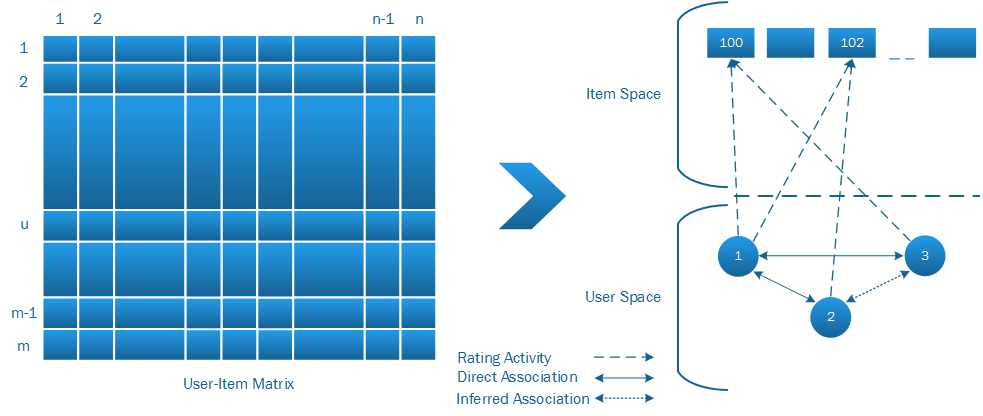
\includegraphics[width=5in]{image/trustnetwork.png}
    \centering
    \caption[Underlying Social Networks in Recommender Systems]{Underlying Social Networks in Recommender Systems}
    \label{figure:cfsocialnetwork}
\end{figure}

Due to the number of ratings that exist in recommendation systems, underlying
social networks are very sparse. There are cases in which insufficient or loss
of information is detrimental for the recommendation algorithms. Consider
Figure \ref{figure:cfsocialnetwork}, classic CF will associate only the users
which have co-rated an item (User $1$ and $2$ and user $1$ and $3$). To deal
with the problem of a sparse social network, it is possible to infer trust
between a source user $S$ and a target user $T$ through an intermediate user
$N$ (User $2$ and $3$ are connected through the intermediary user $1$), as
shown by the \emph{Inferred Association} arrow. According to this process,
trust is propagated in the network and associations between users are built,
even if they have no co-rated item. Trust paths can be of variable length,
depending on the number of associations that one needs to traverse in order to
reach the target user.

% Trust-paths
For example, if the trust $T_{1 \rightarrow 2} = 0.7$ based on 5 co-rated items
and $T_{1 \rightarrow 3} = 0.35$ based on 2 co-rated items, then the trust
between user $2$ and $3$ through $1$ is, $T_{2 \overrightarrow{1} 3} = 0.6$
($\frac{0.7*5}{5+2} + \frac{0.35*2}{7}$)

In order to express the subjective notion of trust, the authors set up a
confidence model that is assigned to each direct association of the network
that expresses the reliability of the association. Confidence is related to the
number of co-rated items between two users. The confidence scores are all
expressed in relation to the most confident association for each user.

\begin{equation}
C_{s \rightarrow t} = \frac{n(I_{s} \cap I_{t}}{n(I_{s} \cap I_{u_{MAX_CONF}}})
\end{equation}

Using the above example, assuming that the maximum number of co-rated items
user $1$ has with any user is 7, $C_{1 \rightarrow 2} = \frac{5}{7}$

% Results/Findings
The authors achieved improved accuracy for all sparsity levels. With a sparsity
level of $99.9\%$ the 2-HOP CF (friend of friends) increased the MAE
performance by $17\%$ over standard CF methods.

% Using a Trust Network to Improve Top-N Recommendation
% Article Comments:
%		-

Jamali et. al. \cite{Jamali2009} propose two different methods for getting
around the cold-start user problem using a trust network.

Their first approach called \emph{Random Walk} only utilize the trust network to provide recommendations. Starting from the active user $u$, we perform a random walk on the trust network. Each
random walk stops at a certain user. Then the items rated highly by that user
will be considered as recommended items, ordered according to the ratings
expressed by that user. We perform several random walks to gather more
information and compute a more confident result. The estimated rating of each
item is the average of ratings for that item over all raters considered. At the
end, we output items with the highest estimated rating as top-N recommended
items.

Their second appraoch called \emph{Combined Approach} uses both user-user similarities and the trust network to provide recommendations. In this approach we compute the top $K$ trusted users in the network and rank
the items rated by these trusted users to compute top-N recommended items. We
use the collaborative filtering approach to compute another set of top-N
recommended items. Finally, we merge these two lists to produce a combined list
of top-N recommended items. The top $K$ trusted users can either be found by
\emph{Breadth First Search} or \emph{Random Walk in the social network}.%d

Their approaches showed great improvements in recall for cold-start users,
improving the performance by 50$\%$ over the standard collaborative filtering
approach. The main improvements however, are the coverage of the trust-based approaches, while still maintaining the same or even slightly better precision than the standard CF methods.

%TODO - READ: A Matrix Factorization Technique with Trust Propagation for Recommendation in Social Networks

\subsubsection{Filterbots}

% Na¨ıve Filterbots for Robust Cold-Start Recommendations

Park et. al. \cite{Park2006} propose using filterbots to improve the cold-start
performance of collaborative filtering methods. Their filterbots are a varition of RipperBots, described in \cite{Good1999}.

A filterbot is an automated agent that rates all or most items using IF techniques. The filterbots injects psuedo
users or bots into the system. These bots rate items algorithmically according to item features and user profiles. For their movie recommendation systems the author propose using 7 global bots which rates movies based on average item rating, a critic bot that generates ratings based on the average critic (pre-selected users) ratings, an award bot that generates rating based on the awards a movie has won, and so on. These ratings generated by these bots are injected into the user-item matrix along with actual user-item ratings. Standard CF algorithms are then applied to generate
recommendations. 

Their approach clearly demonstrated better robustness to all three cold-start situations than standard item-based
and user-based collaborative filtering. The improvements were most evident on
the datasets with a high degree of sparsity.

\subsubsection{Wisdom of the better few / Seed users}

% Wisdom of the Better Few: Cold Start Recommendation via Representative based Rating Elicitation

Liu et. al \cite{Liu2011} propose an approach in which they elect a few
representative users and items. The representative set should represent a set
of active users or items who well represent the entire population but with
little taste overlap. In their approach they wish to find a rank-k
factorization of the form $Y \approx XR$ or $Y \approx CX$ where $X$ is a
loading matrix consisting of free parameters and $R$ and $C$ which is the
component matrix consisting of actual rows or columns from $Y$. The
representative users and items are found using dimensionality reduction
techniques by reducing the column space of the rating matrix from $m$ to $k$.
And then applying basis selection based on the maximum-volume principle to
select the $k$ most representative users or items. In order to be able to
recommend new items to the users it must first be rated by the $k$
representative users, likewise for new users to be rated they need to rate the
$k$ most representative users. Their method therefore easily allows new users
to be \emph{folded in}.


\subsubsection{Intelligent Selection / Interview Process}\mbox{}\\

%My though behind including these articles:
%Use e.g. a tinder like interface and ask the user to like/dislike 15 items when first logging in

\begin{chapquote}[30pt]{Vanessa Redgrave}
  "Ask the right questions if you're going to find the right answers"
\end{chapquote}

% Getting to Know You: Learning New User Preferences in Recommender Systems 
 
As pointed out by Rashid et. al. \cite{Rashid2002}, the most direct way of
acquiring information for use in personalized recommendations from a new users
is to present item for the user to rate. However, they argue that the system
must be careful to present useful items to garner information. A food
recommender should probably not ask whether a new user likes vanilla ice cream
since most people like vanilla ice cream. Therefore, knowing that a new user
likes vanilla ice cream tells you very little about the user. The choice of
what questions to ask a new user, then, is critical. The authors performed a
study of different item selection strategies that collaborative filtering
recommender systems can use to learn about new users. They presented the users
with a questionnaire with items asking them to rate/select the ones they like.
Their strategies can be divided into five classes, which they evaluated based on user effort and accuracy:

\begin{itemize}
\item \emph{Random:} strategies: Strategies that avoid bias in the presentation
of bias
\item \emph{Popularity:} Select among the top N items where the probability
that an item is selected is proportionate to the items popularity.
\item \emph{Pure entropy:} Present the items with the highest entropy that the
user has not seen
\item \emph{Balanced strategies:} A balanced approach combining both popularity
data and entropy.
\item \emph{Personalized:} As soon as some information is known about a user,
present items specifically tailored to that user using e.g. item-item
similarity
\end{itemize}

Their suggestion for an e-commerce recommender system is to start off recommending the most popular
items rather than the highest rated ones, and then use item-item similarity as
quickly as possible.

% Learning preferences of new users in recommender systems: an information theoretic approach

This study was later extended by Rashid et. al. \cite{Rashid2008} where they
more closely examined information theoretic strategies for item selection. In the article they introduced three new strategies, which where compared based on user effort and accuracy:

\begin{itemize}
\item \emph{Entropy0}: Entropy Considering Missing Values
\item \emph{HELF:} Harmonic mean of Entropy and Logarithm of Frequency
\item \emph{IGCN:} Information Gain through Clustered Neighbors
\end{itemize}

It is worth mentioning that the authors worked on the cold-start new user
problem for a movie recommender. The implications of this is that a user must
have watched a movie, in order to rate it. This is not so important for our
domain, as taking a quick look at the item should be sufficient to like/dislike
it. We also currently have no way of calculating entropy as we have no rating distribution for our items.

We are constrained to unobtrusively learn user-profiles from the natural
interactions of users with the system, meaning that we can not require the user
to rate e.g. 10 items before we can start providing recommendations. We
currently have a \emph{mixed initiative} system meaning that there is
provisions for both user and system controlled interactions. We (the system)
can only select which items to recommend to the user, and this does not mean
that the user actually will click an item or rate it. Our rational for including these articles is that we envision a simple "hot or not" interface to be used to present items to new users when the first log in to the system.

% User effort vs. accuracy in rating-based elicitation

Cremonesi et. al. \cite{Cremonesi2012} performed a set of experiments where
they looked at the trade-off between user-effort and accuracy. More
specifically, how many ratings are enough to provide good quality
recommendations to new users? The authors conclusion is that between 5 and 20
ratings are optimal for the movie domain. They concluded that 10
ratings is \emph{enough}, but that this number depends on the recommendation method
and the dataset used.

\subsubsection{Hybrid Methods}

%TODO - Sort articles, some are more general cold-start solutions (not just new-item)
%TODO - Add some fancy math, wait until matrix factorization intro is in place (so we do not mess up notations)
%TODO - Find some sweet cf articles incorporating demographic information
%TODO - Merge the hybrid sections fro all subsubsections?

Another line of search for solving the cold-start problem is to utilize features of items and users. The content features can be used to capture the similarities between users and items, thus reducing the amount of data required to make accurate predictions. User data that may be collected typically includes age, gender, nationality, marital status, income, educational level and occupation. Item data could e.g. be the price of a product, title, description, editorial ratings and so.

%The idea is that people with a more common background share a more similar taste than someone with a random background, and therefore good %recommendations can be made as long as we know the new user’s background. 

This section will present some latent factor models presented recently proposed that incorporate both user/item features and past interactions. In Matrix factorization methods, the regularization is mostly based on a
zero-mean Gaussian prior on the factors, we refer to this method as ZeroMean. However. in these models the dyadic response matrix $Y$ is estimated by a altent factor model such that $Y \approx U^{T}V$, where the latent factor matrices, $U$ and $V$, are estimated by regression such that $U \approx FX$ and $V \approx MZ$. $X$ and $Z$ denote user attribute and item feature matrices, and $F$ and $M$ are weight matrices learned by regression. The difference between these methods are how they estimate the weights.

% Regression-based Latent Factor Models

Agarwal et. al. \cite{Agarwal2009} propose a class of latent factors models
called regression-based latent factor model (RLFM) that incorporates both user/item features and past interaction data
into a single model. Their approach utilizes features of items and users as the
prior distribution for latent profiles in matrix factorization.

Users and items are anchored around a global feature-based one where profiles are constructed by estimating deviations from the global ones in a smooth fashion. The deviation depends on the amount of information available, e.g. items/users with sparse data are aggressively "shrunk" to the global one. New items and users start out with profiles based on their known features that gets refined smoothly with the availability of more data. 

Regularizing latent factors through regression has important consequences when modeling sparse dyadic data. For users/items with little data, one obtain reliable factor estimates by using the regression estimates as a fallback. This allows the model to effectively deal with both cold start and warm start situations.

% fLDA: Matrix Factorization through Latent Dirichlet Allocation
%

Agarwal et. al \cite{Agarwal2010} propose a Matrix factorization method to predict ratings in recommender system
applications where a "bag-of-words" representation of item meta-data is natural. Their method regularizes both user and item factor simultaneously through user features and the bag of words associated with each item.

The key idea of their method is to let user factors take values in an Euclidean space of existing factorization models, but assign item factors through a richer prior based on Latent Dirichlet Allocation (LDA). The main idea behind LDA is to attach a discrete latent factor to each word of an item that can take $K$ different values ($K$-topics) and produce item topics by averaging the per-word topics in the item. An article where 80$\%$ of the words are assigned to politics and the rest to education would be though of as a political article related to the issue of education. This allows us to model the affinity between user $i$ and item $j$ as $s'{j}\hat{z_{j}}$, where $\hat{z_{j]}$ is the multinomial probability vector representing the soft cluster membership score of of item $j$ to the $K$ different latent topics. 

% Matchbox: Large Scale Bayesian Recommendations
% 	Online algorithm

Stern et. al. \cite{Stern2009} presents a probabilistic model called Matchbox. The system makes use of content information in the form of user and
item meta data in combination with collaborative filtering information from previous user behavior in order to predict the value of an item for a user. Much like \cite{Agarwal2009} the factors are regularized by incorporating more flexibility in the Gaussian priors through regression on user and item factors.

Their model is dynamic, meaning that it allows an item's popularity, a user's taste or user's personal rating scale to drift over time, as well as being training online. This means that the value of weight matrices $F$ and $M$ will drift over time, this is accomplished by the addition of Gaussian noise each time step. Inference is accomplished a combination of message passing and expectation propagation.

% Learning Attribute-to-Feature Mappings for Cold-Start Recommendations
% 	Model for positive implicit feedback!
% 	Demonstrates usefulness for new-item recommendations
% 	See A. Item Recommendation from Implicit Feedback in the article for implicit feedback recommendations
%	k-NN worked best with MORE features than the linear mapping functions
%	Code can be found at: ismll.de/mymedialite

Gantner et. al. \cite{Ganter2010} propose a method on how to map additional
information such as user and item features to the latent features of a matrix
(or higher dimensional) factorization model. At the core of their approach is a
standard factorization model, optimized to the recommendation task. The
extensions include a mapping function that compute adequate latent
representations for new entities from their attribute representations. This
mapping function could allow new items and users latent features to be found
only based on content-information and further on be used as if they were
normally trained latent features. The training of the factorization model with
a mapping extension consists of the following steps:

\begin{enumerate}
\item training the factorization model using the data $S$, and then
\item learning the mapping functions from the latent features of the entities in the training data and their content attributes
\end{enumerate}

The authors use BPR-MF, a matrix factorization model based on the Bayesian Personalized Ranking (BPR) framework as their factorization model. The authors experimented with two different ways of mapping item/user attributes to the factor space (Only attribute-to-feature mapping for items are presented in the article):

\begin{enumerate}
\item k-NN Mapping:	Weighted k-NN regression for each factor. Determine the k-nearest neighbors as the most similar items according to the cosine similarity of the attribute vectors.
\item Linear Mapping: Each item factor is expressed by a weighted sum of the item attributes. Suitable parameters for the mapping function is learned by optimizing the model for the squared error on latent features.


\subsection{Fashion Recommendation}


\subsubsection{Theory}
This subsection will look into some background research on fashion.
And look into what fashion is and why a consumer behaves like the consumer does.

\textbf{What is fashion:}
There are a lot of different ways of defining what fashion really is.

\begin{itemize}
    \item Some claim it to be the entire spectrum of attractive clothes at any given time.
    \item Others may claim it to be the worship and pursuit in an era or at one
    time.
    \item In \cite{Fang2012} this definition on fashion is being used: "Fashion is
    the social norm recognized and advocated by a particular social class at one
    time. It affects all the fields in society, especially and famously in
    clothing. Sometimes, short-lived fashion is referred to as style."
    \label{items:fashionDefinitions}
\end{itemize}

As seen from the different definitions mentioned above, what is reoccurring is;
clothes, popularity, time and a cultural grouping.
\todo{Better flow}
enough items to make the assumption

\textbf{Task of fashion marketing:}
Fashion is subject to constant change as seen from the different definitions of fashion from ~\ref{items:fashionDefinitions}.
Some of these changes are due to human changes such as adoption of a new line of clothing, or something less controllable, such as the changing of the seasons.
How much of a product should be made to satisfy the need of the consumer, but still remain a desirable product the consumer would find itself unique and special with.
What is a reasonable price for the product, and how much is the name of the designer worth?
Who can distribute the product with the product loosing its value and fashion status.
This are just some of the questions the fashion industry has to answer.
Without them answered the potential of the product can't be reached.
Which could lead the consumer not to feel the uniqueness and prestige of the item.
Fashion trends comes and goes, and the new fashion starts with the refusal of what is old.

% Companies must: MTODO Not interesting in our case?
% - find consumer needs
% - consumer segment, how to approach
% - pos to reach segment
% - reqs of the segment
% - price
% - channel distribution demands
% - sails starts at segment

In fashion there is a big difference between men and women in what, where, when
and how they buy.  How to understand the behavior of the consumers and how they
act can come from a vast set of areas, the main factors influencing the consumer according to \cite{kotler2009marketing} is:

\begin{table}[H]
    \centering
    \begin{tabular}{l|l|l}
      \textbf{Factors}        & \textbf{Examples} & \textbf{something?} \\ \hline
      Physiological factors   & Physical protection, commodity & - \\ \hline
      Socio-cultural factors  & Family, friends, work, social groups & - \\ \hline
      Personal factors        & Age, life cycle, occupation, personality & - \\ \hline
      Psychological factors   & Product reliance or sympathy & - \\ \hline % more expensive because more expensive - increase self-confidence
      Rational factors        & Brand of product, quality, designer, price & - \\
    \end{tabular}
    \label{table:FashionFactors}
    \caption [Fashion Factors]{Main factors influencing the consumer when it comes to their buying behavior}
\end{table}
\todo{Last column for in depth explanation (perhaps)}
When it comes to fashion it is mainly a socio-cultural phenomenon.

One central factor when it comes to shopping and fashion is price, a rational factor.
The consumer acts rational, when it comes to price and quality~\cite{Hanf1994}.
In the case of fashion, and a product connected with prestige, this rational behavior might not apply.

There is a set of product criterias a consumer evaluates when it comes to the acquisition of a product~\cite{dutton2006}, attributes found to have the most significant impact was styling, brand , price, place(store), fabrication/fiber content.

\begin{table}[H]
    \centering
    \begin{tabular}{l|l|l}
      \multicolumn{2}{c|}{\textbf{Concrete Attributes}} & \textbf{Abstract Attributes} \\
      \multicolumn{2}{c|}{\textbf{(product features)}} & \multirow{2}{*}{\textbf{(attitude-based)}} \\ \cline{1-2}
      Intrinsic (hedonic)   & Extrinsic & \\ \hline
      \pbox{4cm}{
          - Style \\
          - Color \\
          - Patten \\
          - Fabric/fiber \\
          - Appearance \\
          - Fashionability \\
          - Durability \\
          - Comfort \\
          - Quality \\
          - Fit \\
          - Care \\
      } & \pbox{6cm}{
          - Price \\
          - Brand \\
          - Country of origin \\
          - Place(Store) \\
          - Salespeson's evaluation \\
          - Approval of others \\
          - Coordination with wardrobe \\
      } & \pbox{4cm}{
          - Fun \\
          - Entertainment \\
          - Enjoyment \\
          - Need \\
          - Function \\
        } \\ \hline
    \end{tabular}
    \label{table:ConsumersPurchaseDec}
    \caption [Consumers' Purchase Decisions]{The attributes effecting the consumer when in the process of consuming products~\cite{dutton2006}}
\end{table}

The modern consumer finds pleasure with consumption experience itself, not just the product, and this especially applies to the fashion domain.
The purchase is often not done by need, but for pleasure.

\textbf{Consumer buying behavior:}
A lot of information about the consumers behavior is lost due to the reasons for their behavior is held in an unconscious or implicit level.
The reason for a person is interested in a specific product could be based on some distant memory of the consumers life.
This could affect how a consumer views a particular brand or product for good or worse.
Brand choices are often made intuitively, based on their subconscious, and cannot tell why they mad that choice.

Culture is one of the main factors to determine consumer behavior.
Culture can be segmented into three parts: Culture, subculture and social class.
All consumers are included in many smaller subcultures such as nationality, religious subcultures and geographical subcultures.
Subcultures can be a efficient way of constructing marketing campaigns and aim similar products at, since they tend to form market segments.
The forming of a subculture happens through individuals seeking out other individuals with similar tastes regarding a variety of aspects~\cite{vignali2009fashion}.
There are a lot of different behavior emerging from subcultures, such as peer pressure.
Social psychology is used to understand the behavior of the individuals in subcultures~\cite{vignali2009fashion}.

\textbf{Customer satisfaction:}
There are two main concepts when it comes to customer satisfaction:
Transaction specific and cumulative specific.
The transaction specific satisfaction of the consumer is base on the expectations in the pre-purchase stage and the perceived performance of the product in the post-purchase stage.
Where the cumulative looks at the purchase as a whole, such as: the product, the purchase and the service received~\cite{kumari2012}.
The transaction specific focuses on the post-purchase, if the expectations of the product during the pre-purchase is met in the post-purchase stage, the likeliness of a repeat purchase is increased.



\subsubsection{What Other Fashion Recommender Systems Has Done?}
\todo{A shorter and more precise way of saying this}
This subsection will look methods of other fashion recommender systems and other proposed methods to recommend products in the fashion domain.

\textbf{Photograph based approach}
Fashion and the products it regards are highly dependent on visuals.
A fashion product would not be very interesting if no one saw it. %MTODO redundant?
An approach to use the importance of how the product looks regarding recommending is to utilize images of the product.
Fashion Coordinates Recommender System Using Photographs from Fashion Magazines~\cite{Iwata:2011} is a system doing this.
They teach their system by using fashion magazines with full body images.
They segment the image into two parts, top and bottom.
From this the system learns which top matches to which bottom and collects visual features of the products.
From this the system can recommend other tops to go with a selected bottom, or other way around.
The proposed system scored better\footnote{Accuracy of 50\% on the top 5 suggested items, whereas naive and random managed 18\% and under 5\% respectively} than both a more naive approach and a random selection.
Runtime was at 0.04 seconds per recommendation.


\textbf{Hot-or-not}
A recommender system called SuitUp~\cite{SuitUp} did a survey on some of their potential users.
One interesting finding was that many of the users enjoyed the Hot-or-Not feature of the system.
This feature gives the user a set of items and the option to either like or dislike.

\textbf{Trust based}


% Building Recommender Systems using a Knowledge Base of product semantics
% http://images.accenture.ca/SiteCollectionDocuments/PDF/recommenderws02.pdf
% 	- Would probably require some more product semantics...

%What are the challanges of making recommendations for fashion?

%	- For how long are items relevant?
	%	- Spring, Summer, Fall, Winter collections
			%Improving E-Commerce Recommender Systems by the Identification of Seasonal Products (Article)
	%	- Freshness, fresh decay operators

%	- Implicit feedback (Based around users fashion browsing habits and an occational purchase...)
	%	- What do we look at? What information is the most useful
	%		- Item category, item keywords, brand... ?

%	- Changing interest of users
%	- Unstructured content/multiple content providers
	% - How to select features for a content-based approach
		% E.g. keywords, when descriptions are in multiple languages
%	- Sparsity
	% - Can rating infromation from similar items be used to decrease sparsity? (Content infromation - Hybrid approaches)
%	- Trends?
	%	- How important is e.g. item popularity?

\subsection{Recommender Systems (general)} %MTOD naming
\subsubsection{Collaborative Filtering}
In collaborative filtering the system will utilize the other users and the user's ratings to make predictions. \todo{maybe maybe ambiguous}
Ratings can be based on a variety of feedback from the user, such as: rating from 1 to 5, like or dislike, having a look at an item or buying an item.
For each user, in a collaborative filtering system, there will be a set ratings, for the more active users the amount of ratings will be higher.

\textbf{Recommendation}
The prediction of items for a user is done through looking at the user and other users.
The system will try to find similar users based on the other users ratings.
Based on this subset of users, the system can predict items by suggesting new items the user is not familiar with, but similar users have shown interest in. \todo{ambiguous who the user is?}

There are a lot of algorithms used in the field of collaborative filtering to find and recommend items. This can be divided into two categories: Memory-based and Model-base algorithms.

\missingfigure{some awesome CF image}

\textbf{Memory-based}
In memory based collaborative filtering the entire user-item database is used to generate recommendations.
A usual approach to find a rating is to look at a set of the most similar users based on their ratings, the user's neighbors, and use the similarity to weight their rating on the item or items in question.
\todo{some awesome CF equation to predict rating}

How to calculate the similarity of users can be done in a variety of ways.
Most of them base their similarity measure on the user's ratings.
Two often used approaches to calculate this is through Pearson correlation coefficient or cosine similarity.
\missingfigure{similarity figure perhaps}

\todo{some more words on memory, and the similarity measure}


\textbf{Model-base algorithms}
As the name implies this approach tries to model the user ratings.
With this approach the complete dataset is not necessary when making predictions, like the memory-based approach often needs.
So instead of using the complete dataset the model is used.
Often used collaborative filtering algorithms to build these models are: Bayesian networks, clustering models, singular value decomposition and Markov decision process based models.


\todo{some more words on model}
\missingfigure{ALS-figure perhaps}


\subsubsection{Content Based Filtering}
\textbf{User Profiling}
In content based filtering the system will utilize the metadata(content) of the item to suggest items with similar metadata or properties.
Based on the items the user previously have rated, either through implicit or explicit feedback, the system can build a user profile for the user.
This user profile is usually a vector of some sort representing the users preferences through weighting the collected item properties from previous ratings.

\textbf{Recommendation}
With this profile the system will try to recommend items for the user.
This is done through matching the profile vector with items metadata.
From this the system produces a level of user interest in the items.
This estimate is used to suggest the items of most interest to the user.

In a fashion recommender system the the set of metadata to an item could be attributes such as: color, brand, store, size, key words and price.
When recommending items for a user, the items with the most similar metadata to the user's user profile will be suggested.

\missingfigure{maybe some trendy CBF image}

\subsection{Session Based Approach}
\todo{This subsection has been dead for a while. Just here in case of revival (time)}
Init Hypothesis:
Two users with similar session habits and similar product accessing pattern
have a stronger correlation to one-another than two users with just similar
product interests.


'product\_purchase\_intended' (user pushed to the product web store) shows a
wider specter of information about the product, including additional colors,
images and colors.  For some it might be natural to explore the item there
before "wanting" it. Making both

"product\_purchase\_intended" $\Rightarrow$ "product\_wanted"

and

"product\_purchase\_intended" $\notimplies$ "product\_wanted"

produce valuable information.

Must make different rules for the different stores:
"Bik Bok", "Cubus", "Gina Trik", "H\&M", "Bianco" has a broad specter of extra
functions inside the web store, whereas others might not, only shows the
product and a add to chart button.  This might divide the use pattern of the
users into a:

"product\_detail\_clicked" $\Rightarrow$ "product\_purchase\_intended" $\Rightarrow$ "product\_wanted"

"product\_detail\_clicked" $\Rightarrow$ "product\_purchase\_intended" $\notimplies$ "product\_wanted",

and

"product\_detail\_clicked" $\Rightarrow$ "product\_wanted"

based on the store accessed.

Use this to make a "rule set" with a probability.
Then again use this to recommend items for the users with that given
probability.

Find a "most popular session"-pattern
Find a "most likely to come after"-pattern

% db.sessions.group({key:{'storefront_name':1},cond:{},reduce:function(cur,result){result.count += 1}, initial: {count:0}})

Articles 4 l8er:
%http://dl.acm.org/citation.cfm?id=1136004
%http://link.springer.com/chapter/10.1007/3-540-46119-1_42
%http://dl.acm.org/citation.cfm?id=1082567
%http://link.springer.com/chapter/10.1007%2F978-3-540-30214-8_20
%http://dl.acm.org/citation.cfm?id=502935
%http://dl.acm.org/citation.cfm?id=1835896
%http://dl.acm.org/citation.cfm?id=345169
%http://dl.acm.org/citation.cfm?id=345169

Session issues:
Once in a blue moon a user will do a "product action" (purchase,want,details)
without having a previous frontstore-access event. Which leads to unknown
store-id of the item.

Issue is most probably from missing user-id in collection\_viewed, and a user
checks out an item from there. It is not possible to be 100\% sure which user
access the item from the collection\_viewed event, so this event is therefor
not integrated into the session-stack.


% thoughts:
Categorize stores
    prize
    items in store

Categorize items
    Type
    Prize
    View frequency

Predicting events...
    Value brought vs. clustering on the "item"-events value

Make a store

% event_id, events:

% Products:
%     "product_detail_clicked",
%     "product_wanted",
%     "wantlist_menu_entry_clicked"
%     "product_purchase_intended",

% Store clicked: (produces not NULL storefront_name) (db.sessions.find({'storefront_name':{$ne:'NULL'},$or:[{'event_id':'featured_storefront_clicked'},{event_id:'storefront_clicked'}]}).count())
%     "storefront_clicked",
%     "featured_storefront_clicked",

% Other store interactions
%     "store_clicked",
%     "around_me_clicked",
%     "stores_map_clicked",
%     "collection_viewed",
%     "featured_collection_clicked",

% Start:
%     "app_first_started",
%     "app_became_active",
%     "app_started",
%     "user_logged_in",
%     "facebook_login_failed",

% Other:
%     "friend_invited",he users rat
%     "activity_clicked",
%     "facebook_share_changed",

% Course:
%     App started
%     Check next events, a days timeframe


%Simple session form, no structure:
% {u'event_id': u'product_detail_clicked', u'count': 68.0}
% {u'event_id': u'product_wanted', u'count': 35.0}
% {u'event_id': u'storefront_clicked', u'count': 69.0}
% {u'event_id': u'app_started', u'count': 26.0}
% {u'event_id': u'featured_storefront_clicked', u'count': 4.0}
% {u'event_id': u'user_logged_in', u'count': 9.0}
% {u'event_id': u'product_purchase_intended', u'count': 2.0}
% {u'event_id': u'around_me_clicked', u'count': 7.0}
% {u'event_id': u'stores_map_clicked', u'count': 1.0}
% {u'event_id': u'store_clicked', u'count': 1.0}
% {'user_id': 100001385800886L}
% {'num_events': 222}
% Total amount:    222
% User:            100001385800886
% Total Sessions:  30
% Total Events:    936
% Date:            11 - 10 - 2013

% Structured session exploration: Probably more info in this
% > db.sessions.find({'user_id':1094505588,session:64},{'event_id':1,'server_time_stamp':1,'_id':0}).sort({'ts':1})

% > db.sessions.find({'user_id':100000140823565,session:440},{'event_id':1,'server_time_stamp':1,'_id':0}).sort({'ts':1})

% > db.sessions.find({'user_id':100000140823565,session:440},{'product_id':1,'event_id':1,'_id':0}).sort({'ts':1})

\subsection{Items clustering}
\subsection{One-Class Collaborative Filtering}

% []
% PDF:
% cite:
% ## Keywords / Short summary

% ## Interesting findings

% ## Quotes

% ## Interesting references literature





% [Implicit feedback] asdfasdf 7.3
% PDF:

% cite:
% ## Keywords / Short summary
% Lot of references to work done on implicit feed back to check out


% ## Interesting findings

% ## Quotes

% ## Interesting references literature
